\chapter{Umsetzung}

	
Nachdem im vorherigen Kapitel die technischen Grundlagen erläutert wurden, wird nun auf die Umsetzung eingegangen. Es wird mit der Umgesetzten Architektur begonnen, um einen groben Überblick über die einzelnen Komponenten zu bekommen. Anschließend wird genauer auf zwei wesendliche Teile eingegangen:
	
\paragraph{Datenhaltung und Anbindung an eine Datenbank}
In diesem Abschnitt wird die Datenhaltung auf dem Handy beschrieben. Dabei wird auf zwei unterschiedliche Methoden eingegangen, die bei der Umsetzung zum Einsatz kamen.
In diesem Kapitel wird auf die Datenbankanbindung an den Server eingegangen. Besonders wird hier auf die verschiedenen Tabellen der Datenbank bezug genommen und das allgemeine vorgehen beschrieben, Daten vom Server zu Laden und dort zu Speichern.
		
\paragraph{Bestandteile der App}
In diesem Abschnitt wird sich mit den generellem Aufbau der App befasst und teilt sich in zwei weitere Teile auf. in Teil eins wir auf die Benutzerschnittstelle eingegangen und die Benutzeroberfläche von NoRPG erklärt. Im zweiten Teil wird auf weitere wichtige Bestandteile der App eingegangen, darunter wichtige Klassen, welche für die App unverzichtbar sind.
	
\section{Architektur}
	
Die Architektur entspricht dem Controller Prinzip, bei dem es eine zentrale Schnittstelle einen Controller gibt. In diesem Fall ist das die Klasse GameControl.cs, welche den Datenzugriff
zwischen App und Server regelt und innerhalb der App alle wichtigen Abhängigkeiten wiederspiegelt. Diese Klasse ist darüber hinaus auch die zentrale Stelle zum speichern und laden von Daten. In Abbildung \ref{architecture} ist die Architektur grafisch dargestellt.


			\begin{figure}[htbp]
				\centering 
				\label{architecture}
				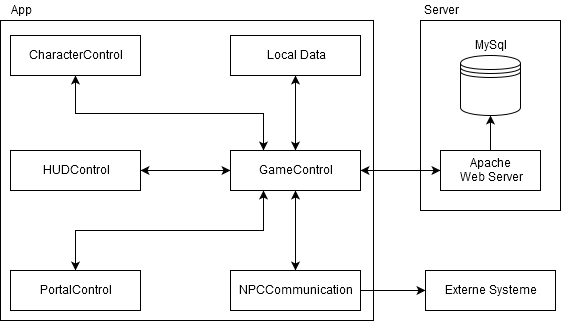
\includegraphics[width=13cm]{pics/archtecture.png}
				\caption{Softwarearchitektur}
			\end{figure}	
			
Darauf ist zu erkennen, dass die Klasse GameController.cs eine zentralle Rolle in der App spielt und im Mittelpunkt steht. Auf dem Server steht eine MySql Datenbank bereit, welche sich um die persistente Datenhaltung kümmert. Neben GameController.cs ist der NPCCommunicationController die einzige Klasse, welche außerhalb der eigentlichen Applikation kommuniziert. Das tut sie mit einem JSON Parser Plugin, welches beim auslesen der JSON Dateinen hilfe(siehe Kapitel \ref{npctext}).	

\section{Datenhaltung und Anbindung an eine Datenbank}

In diesem Kapitel wird die Datenhaltung auf dem Handy und dem Server erläutert. Begonnen wird dabei mit der Beschreibung der Datenhaltung auf dem Handy. Dabei wird auf verschiedene Aspekte der Speicherung eingegangen.

\subsection{Datenhaltung auf dem Handy}

Die Daten auf dem Handy werden im JSON-File Format gespeichert. Es gibt zwei verschiedene JSON Dateien in der App, eines für die Standards, welches vom Server geladen wird, und eines für die Texte der NPCs. Beide Dateien werden unterschiedlich ausgelesen und genutzt. Zuerst wird auf die Standards eingegangen und anschleißend auf die Verarbeitung der Datei mit Texten der NPCs. 
	
\subsubsection{Standards JSON}
Die JSON für die Standards ist ein wichtiger Bestandteil des Spieles. In dieser Datei befinden sich alle wichtigen Infos zu den Standards und deren dazugehörigen Spiele. Diese Datei liegt Zentral auf einem Server und kann dort gewartet und gepflegt werden. Dadurch ist es möglich, zusätzliche Standards und Spiele einzufügen, ohne das der Nutzer die App aktuallisieren muss. Nun wird der grobe Ablauf, gefolgt von einer detailierten Beschreibung, erklärt und beschrieben.
	
			Damit der Nutzer die aktuelle Datei zur Verfügung hat, versucht das Spiel eine zu Beginn eine Verbindung zu dem Server aufzubauen. Gelingt dies, wird die Datei von Server geladen und auf dem Handy gespeichert. Nachdem die Datei gespeichert wurde, wird sie in das Spiel geladen. Dazu wird aus dem JSON eine Liste erstellt, welche überall im Spiel nutzbar ist.
	
			Für das Laden und verarbeiten sind fünf Klassen verantwortlich. Im Folgenden wird nur deatiliert auf die Klasse WebJSONConfigReader eingegangen. Die anderen Klassen sind im Anhang abgebildet und werden nur erwähnt.
	
			Die Klasse MappingStandardsToCourses ist die Datenhaltungsklasse. In dieser ist die Struktur der einzelnen Objekte geregelt. In der Klasse MappingStandardsToCoursesBean spiegelt die Struktur der JSON-Datei wieder. 
	
			Der WebJSONConfigReader wird in der Klasse LoadingScreen genutzt. Dort wird eine Instanz dieser Klasse erzeugt und es wird die Methode LoadSettings ausgeführt und in der Variable Settings gespeichert. Diese Methode ist in Listing \ref{lst:methode3} zu sehen.

\begin{scriptsize}
\lstset{
	float,
	caption=Methode LoadSettings, 
	language=[Sharp]C, 
	frame=single,  
	showstringspaces=false, 
	showspaces=false, 
	numbers=left, 
	captionpos=b, 
	belowcaptionskip=4pt,
	basicstyle=\ttfamily
} 
\begin{lstlisting}[label=lst:methode3]

public MappingStandardsToCourses LoadSettings() {

 WWW www = new WWW(settingsURL);
 while (!www.isDone) { }
  string json;
  string LocalFilePath = Application.persistentDataPath + "/v1.json";

  if (string.IsNullOrEmpty(www.error)) {
   json = www.text;
   File.WriteAllText(LocalFilePath, json);
  } else if (File.Exists(LocalFilePath)) {
   json = File.ReadAllText(LocalFilePath);
  } else {
   json = "";                
   File.WriteAllText(LocalFilePath, json);
  }
  Debug.Log(json.ToString());
  MappingStandardsToCoursesBean settingsBean = 
  		MappingStandardsToCoursesBean.CreateFromJSON(json);
  string json2 = JsonUtility.ToJson(settingsBean);
  Debug.Log(json2.ToString());

  List<Classes> classes = new List<Classes>();
  foreach (var classe in settingsBean.classes) {
   List<Courses> courses = new List<Courses>();
   foreach (var course in classe.courses) {
    List<Standards> standards = new List<Standards>();
    foreach (var standard in course.standards) {
     List<Games> games = new List<Games>();
     List<string> vor = new List<string>();
     List<string> nach = new List<string>();
     foreach (var game in standard.games) {
      games.Add(new Games(game.id, game.name, game.url));
     }
     foreach (var vorbedingung in standard.vorbedingungen) {
      vor.Add(vorbedingung);
     }
     foreach (var nachbedingung in standard.nachbedingungen) {
      nach.Add(nachbedingung);
     }
     Games[] g = games.ToArray();
     string[] v = vor.ToArray();
     string[] n = nach.ToArray();
     standards.Add(new Standards(standard.name, v, n, g));
    }
    Standards[] s = standards.ToArray();
    courses.Add(new Courses(course.name, s));
   }
   Courses[] c = courses.ToArray();
   classes.Add(new Classes(classe.name, c));
  }
  Classes[] cla = classes.ToArray();
  return new MappingStandardsToCourses(cla);
 }
\end{lstlisting}
\end{scriptsize}

In dieser wird zu Beginn ein neues WWW Objekt erstellt. Dieses baut eine Verbindung zum Server auf. Anschließend wird in Zeile 9 überprüft, ob es zu einem Fehler beim Verbindungsaufbau gekommen ist. Wenn es zu keinem Fehler gekommen ist, wird der Inhalt des WWW Objekts in eine Datei geschrieben und gespeichert. Für den Fall das ein Fehler aufgetretten ist und das WWW Objekt keine Verbindung zum Server aufgebaut werden kann, wird geprüft ob bereits eine ältere Datei vorhanden ist, wenn ja, wird der Text aus dieser Datei zum Erzeugen des Objektes genutzt. Anschlißend wird in Zeile 19 aus dem Text eine JSON Struktur erzeugt. Aus dieser wird anschließend in mehreren Schritten ein mehrdimensionaler Array erzeugt und zurückgegeben.

\label{npctext}
\subsubsection{NPCText JSON}
ALI TEXT PLS 

\subsection{Anbindung an einen Server}
Zum Senden der Daten der Registrierung wird das Skript SendDataToServer.cs genutzt. In diesem werden die Daten der Registrierung zwischengespeichert und am Ende an den Server gesendet. Dazu wird die Methode SendRegister() genutzt. In dieser wird die Methode RegisterUser() als Coroutine gestartet. Dazu werden zehn Parameter übergeben, der Username, die Email, das Passwort, der Vorname, der Nachname, das Geburtsdatum, das Geschlecht, der Herkunftsstaat, die native Sprache und der gewählte Charakter. Bei einer Coroutine handelt es sich um einen Thread, welcher beliebig gestarte, pausiert und beendet werden kann.
	
Innerhalb dieser Methode wird zu Beginn ein Hash erstellt, welcher am Server genutzt wird, um zu überprüfen, ob die Anfrage gültig ist. Dieser besteht dabei aus teilen der Eingabe und einem zusätzlichen geheimen Schlüssel, welchem nur der App und dem Server bekannt sind. Dadurch wird die Sicherheit gesteigert und es wird Angreifern erschwert unberechtigte Zugriffe auf die Datenbank zu tätigen. Bei dm Hash handelt es sich dabei um die MD5 verschlüsselten Eingabedaten. Dadurch ist es fast nicht möglich, einen Validen Hash zu bilden, ohne diese Daten zu kennen.
	
Nachdem der Hash erstellt wurde, werden alle Parameter in Form einer Url aneinander gehängt. Anschließend wird die URL an ein WWW Objekt übergeben und solange gewartet, bis es eine Antwort gibt. Sofern es keinen Fehler gab, wird ein Text ausgegeben, welche vom Server gesendet wird, andernfalls eine Fehlermeldung.

\begin{scriptsize}
\lstset{
	float,
	caption=Skript SendDataToServer.cs, 
	language=[Sharp]C, 
	frame=single,  
	showstringspaces=false, 
	showspaces=false, 
	numbers=left, 
	captionpos=b, 
	belowcaptionskip=4pt,
	basicstyle=\ttfamily
} 
\begin{lstlisting}[label=lst:c_SendDataToServer]
using System;
using System.Collections;
using System.Collections.Generic;
using UnityEngine;
using UnityEngine.UI;

public class SendDataToServer : MonoBehaviour {

    private static string secretKey = "norpg";
    public static string registerURL = "http://norpg.it.dh-karlsruhe.de/register.php?";
    public static string loginURL = "http://norpg.it.dh-karlsruhe.de/login.php?";

	...
	...

    private void SendRegister() {
        StartCoroutine(RegisterUser(userText, emailText, MD5Test.Md5Sum(passwordText), 
        	firstnameText, lastnameText, birthdayText, genderText, 
        	countryText, native_languageText, selected_characterText));
    }

    IEnumerator RegisterUser(string user, string email, string password, string firstname, 
    	string lastname, string birthday, string gender, string country, 
    	string native_language, string selected_character) {

        string hash = MD5Test.Md5Sum(user + email + password 
        	+ firstname + country 
        	+ selected_character + secretKey);

        string post_url = registerURL
            + "user=" + WWW.EscapeURL(user)
            + "&email=" + WWW.EscapeURL(email)
            + "&password=" + WWW.EscapeURL(password)
            + "&firstname=" + WWW.EscapeURL(firstname)
            + "&lastname=" + WWW.EscapeURL(lastname)
            + "&birthday=" + WWW.EscapeURL(birthday)
            + "&gender=" + WWW.EscapeURL(gender)
            + "&country=" + WWW.EscapeURL(country)
            + "&native_language=" + WWW.EscapeURL(native_language)
            + "&selected_character=" + WWW.EscapeURL(selected_character)
            + "&hash=" + hash;
        WWW hs_post = new WWW(post_url);
        yield return hs_post;

        if (hs_post.error != null) {
            print("There was an error posting the high score: " + hs_post.error);
        } else {
            status.text = hs_post.text;
        }
    }
}

\end{lstlisting}
\end{scriptsize}
Auf dem Server läuft für die Datenannahme das PHP Skript register.php. Dieses nimmt die Daten aus der URL entgegen und speichert diese zunächst in Variablen ab. Anschließend wird auch in diesem Skript ein Hash gebildet und anschließend mit dem Mitgesendetem abgegleicht. Sollte es hier einen Fehler geben, sendet der Server einen Error zurück, wenn die Hashes identisch sind, wird eine Verbindung zu der Datenbank aufgabenaut und ein Eintrag in der accounts Tabelle erstellt. Anschließend wird eine erfolgreich Meldung an den Client gesendet.

Für den login innerhalb der App wird identisch vorgegangen. Dabei wird jedoch ein Datensatz in die Datenbank geschrieben, sondern nur gelsen. Des weiteren wird der Hash aus nicht so vielen Werten gebildet, da nur der Username und das verschlüsselte Passwort übermittelt werden.